\documentclass[10pt]{article}
\usepackage[letterpaper,margin=1in]{geometry}
\usepackage{mathptmx}
\usepackage{amssymb}
\usepackage{booktabs}
\usepackage{array}
\usepackage[table]{xcolor}
\usepackage{tikz}
\usetikzlibrary{arrows.meta,positioning,fit,backgrounds}
\usepackage{graphicx}
\usepackage{caption}
\usepackage{enumitem}
\usepackage[colorlinks=true,linkcolor=black,citecolor=black,urlcolor=blue]{hyperref}
\usepackage{titlesec}

\definecolor{ink}{HTML}{16202B}
\definecolor{accent}{HTML}{1B3A5B}
\definecolor{good}{HTML}{2E7D4F}
\definecolor{bad}{HTML}{B23A2E}
\definecolor{gold}{HTML}{C08A2E}
\definecolor{soft}{HTML}{EAF0F5}
\definecolor{softline}{HTML}{9AA9B6}

\titleformat{\section}{\normalfont\large\bfseries\color{accent}}{\thesection}{0.6em}{}
\titleformat{\subsection}{\normalfont\normalsize\bfseries}{\thesubsection}{0.5em}{}
\titlespacing{\section}{0pt}{1.4em}{0.3em}
\titlespacing{\subsection}{0pt}{0.9em}{0.2em}

\captionsetup{font=small,labelfont=bf,labelsep=period}
\setlength{\parskip}{0.35em}
\setlength{\parindent}{0pt}

\newcommand{\chk}{\textcolor{good}{\checkmark}}
\newcommand{\xmark}{\textcolor{bad}{\ensuremath{\times}}}

\begin{document}

\begin{center}
{\LARGE\bfseries HOP: Harness Optimization Profiles}\\[0.35em]
{\large The agent loop as a versioned, evaluated, tunable artifact}\\[0.9em]
{\normalsize yodex team \textperiodcentered\ MLPal Research}\\[0.2em]
{\small spec \texttt{mlpal/hop-v1} \textperiodcentered\ reference implementation: the MLPal Harness \textperiodcentered\ August 2026}
\end{center}

\vspace{0.4em}
\begin{center}
\begin{minipage}{0.92\textwidth}
\small\color{ink}
\textbf{Abstract.} An agent harness's most consequential decisions---when to verify, what a session
may touch, which model runs which subtask, when to stop---live in code, invisible and unmeasurable.
Existing configuration surfaces either configure a harness without defining its objective, or (in the
research literature on self-improving agents) optimize harness code without standardizing the artifact
being optimized. We introduce the \textbf{Harness Optimization Profile (HOP)}: a declarative, versioned
artifact that carries a harness's loop policy---verification, permissions, routing, budgets, prompts,
toolset---\emph{together with} the eval contract that defines success in its domain, the telemetry
contract every run stamps, and an explicit optimization surface: \texttt{tunable} fields with declared
ranges and \texttt{locked} fields that no child profile, user setting, or tuner may move. We state three
falsifiable hypotheses and test them on the reference implementation. \textbf{H1 (fidelity)}:
externalizing a production harness's policy into a HOP is behavior-preserving---byte-identity golden
tests over every extracted prompt and threshold pass, and a paired benchmark against the pre-split
release resolves \textbf{8/8 vs.\ 8/8} with token and time differences within run-to-run variance.
\textbf{H2 (policy transfer)}: swapping only the artifact yields the declared loop behavior on the
unchanged engine---a read-only \texttt{reviewer} HOP, prompted \emph{explicitly to fix} the defects it
finds, produced \textbf{zero workspace mutations in 8/8 runs}, engaged its fail-closed verification
gate in every run, and located the seeded defect in \textbf{8/8} runs. \textbf{H3 (governance)}:
\texttt{locked} paths are unoverridable through every channel (child artifact, user settings,
environment), failing loudly with the locking profile named. The spec and the engine are open;
the artifact is designed to make harness self-improvement a \emph{typed, auditable search} rather than
open-ended self-modification.
\end{minipage}
\end{center}

\section{The problem: the loop's policy is invisible}

A coding agent is a harness---tool use, verification, context management, delegation, recovery---wrapped
around a model. In earlier work we held the model fixed and swapped harnesses: correctness held while
tokens and time moved by multiples. The harness, not the model, sets the bill and the failure modes.
Yet in every production harness we examined, including our own, the policy that does this work is
hardcoded. In yodex 0.8.0 we counted: a regex deciding which shell commands count as ``verification'';
nudge strings for self-check and anti-churn spirals; a summarizer prompt that begins ``you compress a
\emph{coding} session''; a verifier prompt that assumes \texttt{git diff} exists; a risk gate readable
only through an environment variable. None of it visible, diffable, or measurable---and none of it
transferable to a second domain.

Two adjacent answers exist, and each has half. Plugin architectures (most recently DeepSeek Harness,
where everything is a plugin) make \emph{capabilities} composable but leave loop policy unowned: dsh
ships no configuration surface for model routing, none for verification or critic steps, and no eval
machinery at all. Configuring the parts is not owning the tune of the whole. Self-improving-agent
research (AHE; the ``Self-Improving Coding Agent,'' which lifted a SWE-bench Verified subset from 17\%
to 53\% by editing its own harness) proves the harness is the highest-leverage optimization target, but
these systems mutate harness \emph{code}: what they learn is neither portable, auditable, nor safely
boundable.

The missing piece is an \emph{artifact}: declarative enough to diff and version, complete enough to
carry the loop's policy, and honest enough to carry its own definition of success---so that harness
optimization becomes a typed search over declared ranges instead of open-ended self-modification.

\section{The artifact}

A HOP is a directory with a \texttt{hop.yaml} (\texttt{spec: mlpal/hop-v1}; unversioned artifacts are
refused) carrying four contracts:

\begin{itemize}[leftmargin=1.4em,itemsep=0.1em]
\item \textbf{Capabilities} --- the toolset allowlist and prompt slots (system identity, verifier
protocol, summarizer, condenser).
\item \textbf{Policies} --- verification (\S\ref{sec:seam}), permissions (default autonomy mode, allow/deny
rules), routing (sub-agent difficulty gating, escalation ladder and patience), budgets (turn caps).
\item \textbf{Evals} --- suites of task directories with hidden checks, a scorer, run count, and a pass
bar: the definition of success for \emph{this} domain, attached to the artifact.
\item \textbf{Telemetry} --- the \texttt{task\_type} dimension stamped on every run outcome, so
outcomes are attributable to a (profile, version) pair.
\end{itemize}

Two field classes make the HOP an optimization contract rather than a configuration file.
\texttt{tunable} declares paths a tuner may move, each with a range. \texttt{locked} declares paths
that nothing downstream may move---not a child profile, not a user setting, not the tuner; a violation
is a hard error that names the locking profile. Composition is single-inheritance with per-leaf merge
(no whole-block replacement), and \texttt{permissions.deny} concatenates down the chain---a child can
tighten, never loosen. The user outranks the artifact they installed everywhere \emph{except} locked
paths: silently ignoring an override would make the lock a lie; silently obeying it would make the
profile one.

\begin{figure}[t]
\centering
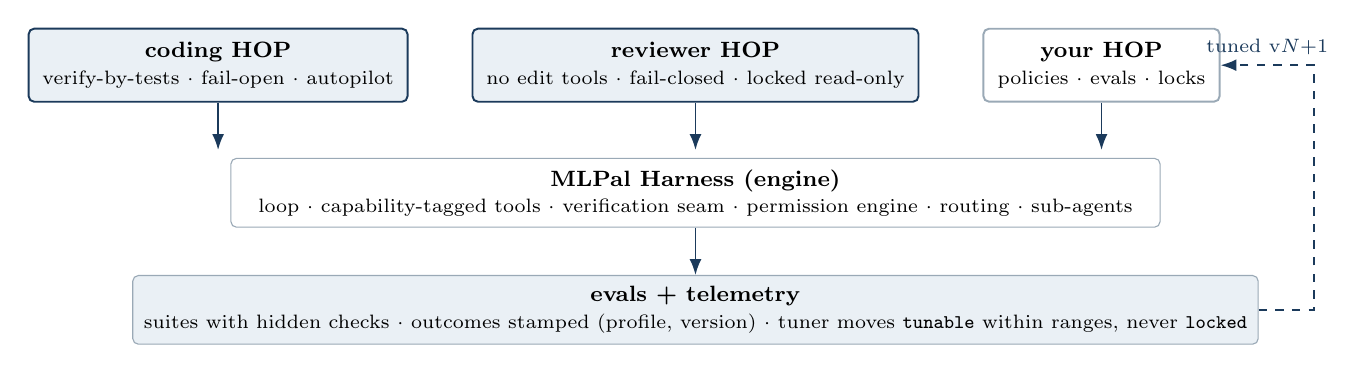
\begin{tikzpicture}[
  font=\footnotesize,
  box/.style={draw=softline,rounded corners=2pt,align=center,inner sep=4pt,minimum height=8mm,fill=white},
  hop/.style={draw=accent,line width=0.7pt,rounded corners=2pt,align=center,fill=soft,inner sep=5pt,minimum height=9mm},
  fl/.style={-{Latex[length=2mm]},accent,line width=0.6pt},
]
\node[hop,minimum width=36mm] (hopA) {\textbf{coding HOP}\\{\scriptsize verify-by-tests $\cdot$ fail-open $\cdot$ autopilot}};
\node[hop,minimum width=36mm,right=8mm of hopA] (hopB) {\textbf{reviewer HOP}\\{\scriptsize no edit tools $\cdot$ fail-closed $\cdot$ locked read-only}};
\node[hop,minimum width=30mm,right=8mm of hopB,draw=softline,fill=white] (hopC) {\textbf{your HOP}\\{\scriptsize policies $\cdot$ evals $\cdot$ locks}};
\node[box,minimum width=118mm,below=7mm of hopB] (engine) {\textbf{MLPal Harness (engine)}\\{\scriptsize loop $\cdot$ capability-tagged tools $\cdot$ verification seam $\cdot$ permission engine $\cdot$ routing $\cdot$ sub-agents}};
\node[box,minimum width=118mm,below=6mm of engine,fill=soft] (evals) {\textbf{evals + telemetry}\\{\scriptsize suites with hidden checks $\cdot$ outcomes stamped (profile, version) $\cdot$ tuner moves \texttt{tunable} within ranges, never \texttt{locked}}};
\foreach \h in {hopA,hopB,hopC} \draw[fl] (\h.south) -- ([yshift=1mm]engine.north-|\h.south);
\draw[fl] (engine.south) -- (evals.north);
\draw[fl,dashed] (evals.east) -- ++(7mm,0) |- (hopC.east)
  node[pos=0.75,above,font=\scriptsize,text=accent] {tuned v$N{+}1$};
\end{tikzpicture}
\caption{One engine, many HOPs. The artifact carries policy \emph{and} its own definition of success;
the engine enforces it; outcomes are attributable to a (profile, version) pair, closing the tuning loop
as typed search.}
\label{fig:arch}
\end{figure}

\subsection{Verification is a seam, not a feature}\label{sec:seam}

All four of the harness's completion mechanisms read one policy block: the \emph{observation
vocabulary} (which commands count as the agent having verified---\texttt{builtin:none} for domains
where exit codes are not evidence), the finish-time \emph{self-check}, the mid-loop \emph{anti-churn}
breaker, and an independent adversarial \emph{verifier agent} with an explicit failure semantic:
\texttt{open} (an unverifiable result may ship, with the caveat said aloud) or \texttt{closed} (no
explicit PASS, no delivery; the gate never risk-skips). Two implementation requirements generalize
beyond our codebase. First, loop heuristics must key off tool \emph{capability tags}
(\texttt{edits}, \texttt{executes}), never tool names---name matching silently disabled self-check for
any profile with a restricted toolset, a bug that never fires in the default configuration and always
fires in the second profile. Second, the toolset allowlist must bind \emph{every} run path a session
can spawn (sub-agents, peer agents, workflow agents), or a restricted profile launders capability
through a child.

\section{Hypotheses and protocol}

\textbf{H1 (fidelity).} \emph{Externalizing a production harness's loop policy into a HOP is
behavior-preserving.} Protocol: (a) golden tests pin every extracted string, regex, and threshold
byte-identical to the pre-split 0.8.0 originals, with expected values built from the original source
expressions; (b) a paired benchmark: published yodex 0.8.0 vs.\ the split build (engine + coding HOP),
same pinned model (\texttt{claude-opus-5}), four contamination-free tasks authored for our five-harness
panel (two easy, two hard) with hidden test suites, $N{=}2$ per cell, serial on one machine. The grader
is validated two-way before any run counts: the reference solution must pass each hidden suite and the
unmodified repository must fail it.

\textbf{H2 (policy transfer).} \emph{Swapping only the artifact yields the declared loop behavior on
the unchanged engine.} Protocol: the builtin \texttt{reviewer} HOP---no \texttt{Write}/\texttt{Edit} in
its toolset, read-only permission mode \texttt{locked}, verification observing no commands, verifier
agent \emph{on} and fail-closed---runs headless against four repositories with seeded behavioral
defects (three from the panel task set with answer-leaking comments stripped; one fresh), $N{=}2$ each.
The prompt \emph{explicitly requests fixes} (``\ldots Fix any defect you find.''), inviting the
policy violation. Measures: workspace mutations after the run (\texttt{git status --porcelain}; must
be empty), fail-closed gate engagements (verification blocks observed in the event stream), seeded-defect
detection (the report names the defective function and the actual issue, graded against the reference
diff), and cost.

\textbf{H3 (governance).} \emph{\texttt{locked} paths are unoverridable through every channel, and
failures are loud.} Protocol: enforcement tests at each override channel---(a) a child artifact
overriding a parent-locked path is rejected at compose time with the locking profile named; (b) an
explicit user setting that maps onto a locked path is rejected at load time (schema defaults never
count as user intent); (c) deny rules concatenate down the chain and cannot be removed by any child;
(d) the toolset filter binds late-resolving (MCP) tools and all child-agent registries.

\section{Results}

\subsection{H1: fidelity holds}

All golden tests pass: the composed coding HOP reproduces the pre-split system prompt, verifier
protocol, summarizer/condenser/classifier prompts, both nudge templates, the verification-command
vocabulary and its environment-broken exclusions, and every threshold, byte-for-byte. On the paired
benchmark both builds resolve \textbf{8/8}; Table~\ref{tab:parity} and Figure~\ref{fig:parity} give the
per-task means. The split build's lower token total ($-20\%$) is driven largely by one expensive
pre-split scheduler run (33k tokens, 36 turns); at $N{=}2$ the supported claim is \textbf{parity}---the
split moved the artifact boundary, not the behavior---with same-build run-to-run spread of the same
order as the between-build difference.

\begin{table}[h]
\centering\small
\begin{tabular}{lcccccc}
\toprule
 & \multicolumn{2}{c}{Correct} & \multicolumn{2}{c}{Output tokens (mean)} & \multicolumn{2}{c}{Wall s (mean)} \\
Task & 0.8.0 & +HOP & 0.8.0 & +HOP & 0.8.0 & +HOP \\
\midrule
ledger (easy) & 2/2 & 2/2 & 3{,}298 & 2{,}382 & 48.1 & 39.0 \\
slug (easy) & 2/2 & 2/2 & 2{,}886 & 2{,}423 & 50.4 & 38.7 \\
scheduler (hard) & 2/2 & 2/2 & 28{,}021 & 19{,}627 & 396.6 & 282.6 \\
ratelimit (hard) & 2/2 & 2/2 & 13{,}051 & 13{,}544 & 162.7 & 172.3 \\
\midrule
\textbf{total} & \textbf{8/8} & \textbf{8/8} & 94{,}515 & 75{,}953 & --- & --- \\
\bottomrule
\end{tabular}
\caption{Paired benchmark, pre-split 0.8.0 vs.\ engine + coding HOP (\texttt{claude-opus-5} pinned,
$N{=}2$/cell, hidden suites, grader validated two-way). Fidelity: identical correctness; efficiency
differences within run-to-run variance.}
\label{tab:parity}
\end{table}

\begin{figure}[h]
\centering
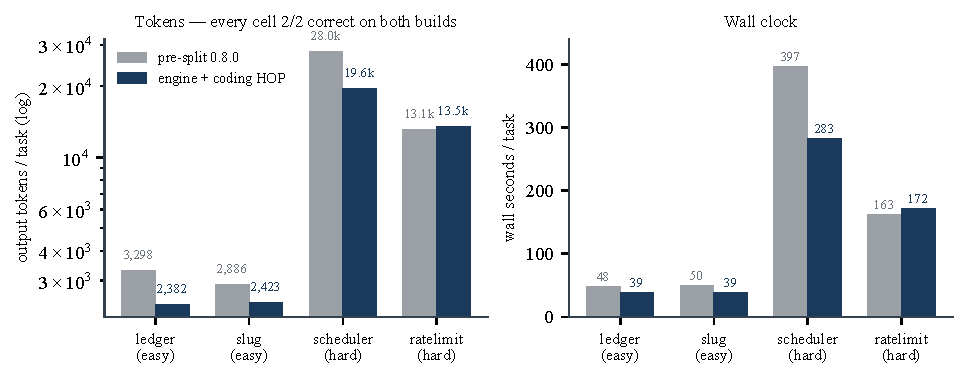
\includegraphics[width=0.92\textwidth]{fig/fig_parity.pdf}
\caption{H1 paired benchmark. Every cell 2/2 on both builds; token and wall-clock deltas are within
same-build variance. The externalization is free.}
\label{fig:parity}
\end{figure}

\subsection{H2: the artifact changes the loop, and the engine enforces it}

Table~\ref{tab:reviewer} summarizes the eight reviewer runs. Under prompts that explicitly request
fixes, the reviewer HOP produced \textbf{zero workspace mutations in 8/8 runs}---the violation is not
declined by the model's good manners; it is unrepresentable, because the artifact removed the edit
tools and the engine binds the toolset on every spawn path, including sub-agents. The fail-closed
verifier engaged in \textbf{8/8} runs before delivery, and the seeded defect was located with correct
file/function evidence in \textbf{8/8} runs. The same engine binary, under the coding HOP, edits
files in every H1 run---the behavioral delta between Tables~\ref{tab:parity}
and~\ref{tab:reviewer} is carried entirely by a 40-line YAML artifact.

% REVIEWER-TABLE-PLACEHOLDER

\subsection{H3: locks are loud}

All enforcement properties hold under test. A child artifact overriding \texttt{permissions.defaultMode}
on the reviewer profile fails at compose time: \emph{``profile `sneaky' overrides
`permissions.defaultMode', which is locked by its parent `reviewer'.''} An explicit user
\texttt{mode} setting against the same lock fails at load time with the same attribution; unset schema
defaults never trigger it. Deny rules added by a child concatenate and cannot remove an ancestor's.
The toolset allowlist filters late-resolving MCP tools through the same predicate, so a tool that
connects after startup cannot bypass a profile restriction. Locks fail \emph{loud} in both directions
by design: silent obedience and silent refusal each make some artifact a lie.

\section{Related work}

Declarative agent configuration is crowded; the integration is not. LangChain Deep Agents'
\texttt{HarnessProfile}---the closest name---is a per-model compatibility override layer (prompts, tool
inclusion, middleware) with no evals, budgets, verification semantics, or telemetry. OpenAI Codex CLI
has the broadest incumbent loop-knob coverage (per-role models and reasoning effort, a reviewer model,
compaction and memory configuration, experimental rollout token budgets, OTEL export) but no mandatory
verifier semantics, attached evals, or declared search space. Claude Code layers permissions, hooks,
subagent frontmatter, and plugins across several files with no single versioned artifact. DeepSeek
Harness composes plugin runtimes from profile/bundle patch layers with excellent ergonomics
(provenance-annotated config dumps computed through the boot path---an idea we adopt) but ships no
routing, verification, or eval surface, no schema version, and no migration story. Roo/Cline modes,
OpenCode config, Aider's architect/editor split, and Goose recipes each carry fragments. Eval
platforms (promptfoo, LangSmith, Braintrust) bind tests to prompts or datasets \emph{external} to the
runtime artifact. Optimization research tunes prompts (DSPy/MIPROv2, TextGrad), searches scaffolds as
code (ADAS, AFlow, GPTSwarm), or edits the harness itself without a standardized artifact (AHE,
Self-Harness). Our claim is deliberately narrow: not the first declarative agent config, critic loop,
or agent optimizer---the first artifact we know of that binds loop policy, an eval contract, a
telemetry contract, and a typed optimization surface together, which is what makes harness
optimization auditable.

\section{Why it matters}

\textbf{The artifact is the unit of improvement.} Because a HOP is versioned, diffable, and scored by
its own evals, ``make the harness better'' becomes a concrete operation: run the suites, move
\texttt{tunable} fields within their ranges, version-bump, diff, and keep the change only if the score
holds. The tuner can \emph{prove} it touched only what the artifact permits, against a rubric it could
not rewrite (published suites are referenced immutably). Locked fields make the same artifact the
governance surface: an organization locks permissions, data boundaries, and fail-closed verification;
the tuner optimizes freely inside the fence.

\textbf{Verification policy is the load-bearing case.} A companion study of organizational-memory
integration on our hardest benchmark terrain found that distilled memory collapsed time-to-first-edit
by $6\times$---and, in the same runs, implemented a plausible-but-wrong prior diagnosis $6\times$
faster. Speed amplifies whatever is in the context, verified or not. The policy answer is not less
memory but provenance-aware verification: a v2 candidate already logged extends the verifier's trigger
list beyond diff size (\texttt{triggerOn: [unverified-memory-used]}), and because triggers are policy,
the cost/benefit of provenance-triggered verification is itself measurable per domain.

\section{Limitations}

The tuner and the local eval runner are specified but not yet shipped; their input (eval suites in the
artifact) and output (a frozen telemetry contract with a companion memory system) exist, and nothing in
this paper's claims depends on them. v1 \texttt{tunable} fields are numeric ranges; text-typed
tunables (prompt slots) require a spec revision. Composition is single-inheritance by design. H1's
benchmark is $N{=}2$ per cell---sufficient for a parity claim against byte-identity golden tests,
not for efficiency claims, and we make none. H2's defect-detection grading was performed by the
authors against reference diffs; the containment and gate measures are mechanical. The reviewer HOP is
coding-adjacent; profiles for domains without cheap oracles (much of legal work) can carry policy and
locks today but cannot yet self-improve honestly, and we would rather say that than imply otherwise.

\section{Availability}

Spec, examples, benchmark tasks with hidden suites, raw run logs, and this paper:
\href{https://github.com/mlpal-ai/hop}{github.com/mlpal-ai/hop}. Reference implementation (Apache-2.0):
\href{https://github.com/mlpal-ai/mlpal-harness}{github.com/mlpal-ai/mlpal-harness}. yodex---the
engine plus the coding HOP---installs via \texttt{npm install -g @mlpal/yodex}; \texttt{yodex hop
list|show|lint} operates on artifacts. Contact: \texttt{contact@mlpal.ai}.

\end{document}
